\documentclass[oneside,senior,etd]{BYUPhys}

\usepackage{cmap} % Для корректной кодировки в pdf
\usepackage[utf8]{inputenc}
\usepackage{rotating}

\usepackage[russian]{babel}
\usepackage{amsfonts} % Пакеты для математических символов и теорем
\usepackage{amstext}
\usepackage{amssymb}
\usepackage{amsthm}
\usepackage{graphicx} % Пакеты для вставки графики
\usepackage{subfig}
\usepackage{color}
\usepackage[unicode]{hyperref}
\usepackage[nottoc]{tocbibind} % Для того, чтобы список литературы отображался в оглавлении
\usepackage{verbatim} % Для вставок заранее подготовленного текста в режиме as-is
\usepackage{listings}

\newcommand{\sectionbreak}{\clearpage} % Раздел с новой станицы

\usepackage{tikz}
\usepackage{pgfplots}
\usetikzlibrary{arrows,positioning}
\usepackage{adjustbox}

\usepackage{makecell}
\usepackage{booktabs}
\usepackage{boldline}

\usepackage{xcolor}
\usepackage{soul}
\usepackage{url}
\usepackage{multirow}
\usepackage{amsmath}

\usepackage{pifont}
\usepackage{indentfirst} % Делать отступ в начале первого параграфа
\usepackage{lscape}

% Общие параметры листингов
\lstset{
  %frame=TB,
  showstringspaces=false,
  tabsize=4,
  basicstyle=\linespread{1.0}\tt\small, % делаем листинги компактнее
  breaklines=true,
  texcl=true, % русские буквы в комментах
  captionpos=b,
  aboveskip=\baselineskip,
  commentstyle=\tt
}

\graphicspath{ {./img/} }

\DeclareMathOperator*{\argmax}{arg\,max}
\DeclareMathOperator*{\argmin}{arg\,min}
\DeclareMathOperator*{\Argmax}{Arg\,max}
\DeclareMathOperator*{\Argmin}{Arg\,min}
\newcommand{\todo}[1]{\textcolor{red}{#1}}

% DEBUG
% \usepackage{showframe}

\Faculty{Факультет вычислительной математики и кибернетики}
\Chair{Кафедра математической статистики}
% Лаборатория
% \Lab{~}
\Year{2025}
  \Month{Месяц}
  \City{Москва}
  \AuthorText{Автор:}
  \Author{Лазар Владислав Игоревич}
  \AuthorEng{Vladislav Lazar}
  \AcadGroup{416}

  \TitleTop{Анализ и применение многофакторных моделей }
  % Раскомментируйте, если нужны еще строчки названия
  \TitleMiddle{динамики лекарственных веществ в медицинских исследованиях}
  % \TitleBottom{Третья строка названия}
  % Uncomment if you need English title
  % \TitleTopEng{Thesis theme, first line}
  % \TitleMiddleEng{Thesis theme, second line}
  % \TitleBottomEng{Thesis theme, third line}

\docname{Выпускная квалификационная работа}
  \Advisor{Захарова Татьяна Валерьевна}
  \AdvisorDegree{кандидат физико-математических наук, доцент\\}
  % Раскомментируйте, чтобы добавить научного консультанта
  %\Consultant{ФИО научного консультанта}
  %\ConsultantDegree{степень, звание\\}

% Закомментируйте, если аннотация не нужна
% \Abstract{
% Аннотация.
% }
% Раскомментируйте, если нужна английская аннотация
% \AbstractEng{Abstract in English}

% Раскомментируйте, чтобы написать благодарности
% \Acknowledgments{Благодарности.}

%%%% DON'T change this. It is here because .sty does not support cyrillic cp properly %%%%
\TitlePageText{Титульная страница}
\University{Московский государственный университет имени М.В.Ломоносова}
\GrText{гр.}
\AdvisorText{Научный руководитель}
\ConsultantText{Научный консультант}
\AbstractText{Аннотация}
\AcknowledgmentsText{Благодарности}
\ListingText{Листинг}
\AlgorithmText{Алгоритм}

% Set PDF title and author
\hypersetup{
  pdftitle={\PDFTitle},
  pdfauthor={\PDFAuthor}
}

\begin{document}
\fixmargins
\makepreliminarypages

\oneandhalfspace

\pdfbookmark[section]{\contentsname}{toc}
\tableofcontents


\section{Введение}
\subsection{Связанные понятия}

\indent \textbf{Фармакокинетика} - раздел фармакологии, ханимающийся изучением воздействия организма на введённый лекарственный препарат. \newline
\indent Под \textbf{биодоступностью} понимают скорость и степень, с которой действующее вещество или активная часть молекулы действующего вещества абсорбируется из лекарственного препарата. \newline
\indent Под \textbf{биоэквивалентностью} двух лекарственных препаратов понимают схожесть их биодоступности.

\subsection{Область исследований}

Процедура проверки биоэквивалентности двух препаратов выглядит следующим образом:

\begin{enumerate}
	\item Набирается группа испытуемых
	\item Каждому испытуемому вводят тестовый препарат
	\item У каждого из испытуемых берут кровь на анализ и определяют концентрацию активного вещества
	\item Процесс повторяют определённое количество раз в течение некоторого времени (интервалы между взятием крови зачастую определены и фиксированы, но в этой работе будем считать их случайными)
	\item Аналогичные действия повторяются с референтным препаратом
	\item Для каждой кривой вычисляется оценка $\textbf{AUC}_{[0; +\infty)}$ (площади под кривой на $\mathbb{R}^{+}$) и получается выборка из $N$ площадей для каждого препарата
	\item Полученные выборки сравнивают с помощью различных критериев биоэквивалентности
\end{enumerate}

Как можно заметить, довольно значительная часть информации о поведении вещества в организме теряется из-за того, что вместо самих кривых используются площади. Так делается по той причине, что о законах, описывающих эти кривые, мало что известно. Поскольку ценой ошибки при проведении подобного тестирования является потенциальное здоровье людей, проблема остаётся до сих пор актуальной. Существуют исследования того, какими способами можно увеличивать точность вычисления площади и снижать вероятность ошибки первого рода. Такие исследования действительно дают результаты, но возможность знать значение концентрации активеного вещества в крови (или же построить в достаточной мере точную оценку) позволила бы построить критерии с меньшей вероятностью ошибки как первого так и второго рода, а значит, снизить потенциальный риск для людей покупающих лекарственные препараты. Целью данной работы является создание математической модели для описания зависимости концентрации от времени и проверка её адекватности на синтетических данных.

\subsection{Постановка задачи}

\begin{enumerate}
	\item Обзор существующих решений
	\item Разработка математической модели описывающей изменение концентрации вещества в крови со временем
	\item Построение оценок на основе полученной модели
	\item Сравнение полученных оценок с уже существующими методами
\end{enumerate}

\section{Обзор существующих решений}

\subsection{$\textbf{PBFTPK}_0$} \label{pbftpk0}

Одним из современых подходов является описанная в \cite{pbftpk} модель \textbf{PBFTPK}. Одним из нововведений является предположение о конечности времени абсорбции (то есть времени, за которое дейстующее вещество распределяется, и после чего его концентрация перестаёт расти). В этой работе авторы, используя уравнения, полученные в \cite{dost}, предложили следующую модель:

\[
	\begin{cases}
		C(t) =  \frac{F D} {V_d} \frac {1}{\tau k_{el}} (1 - e^{-k_{el} t}), & 0 \leq t \leq \tau, \\
		C(t) = C(\tau) e^{-k_{el} (t - \tau)},                               & \tau < t < +\infty
	\end{cases}
\]

где

\begin{itemize}
	\item $C(t)$ - концентрация действующего в момент времени $t$
	\item $D$ - введённая доза
	\item $F$ - биодоступная часть дозы
	\item $V_d$ - объём распределения деуствующего вещества
	\item $k_{el}$ - коэффициент элиминации, отражающий скорость выведения вещества из организма
	\item $\tau$ - время абсорбции
\end{itemize}

Здесь и далее будем называть эту модель $\textbf{PBFTPK}_0$

\subsection{$\textbf{PBFTPK}_1$} \label{pbftpk1}

Модификацией этой модели стала описанная теми же авторами комбинированная модель (здесь и далее - $\textbf{PBFTPK}_1$). В ней этап абсорбции описывается уравнениями из \cite{dost}, а этап элиминации - уравнением из \ref{pbftpk0}. В результате получается следующее уравнение:

\[
	\begin{cases}
		C(t) = \frac{F D}{V_d} \frac{e^{-k_{el}t} - e^{k_a t}}{k_a - k_{el}}, & 0 \leq t \leq \tau, \\
		C(t) = C(\tau) e^{-k_{el} (t - \tau)},                                & \tau < t < +\infty
	\end{cases}
\]


Здесь $k_a$ - коэффициент абсорбции, отвечающий за скорость всасывания вещества в кровь и ткани организма.

Здесь и далее условимся называть отрезок $[0; \tau]$ \textbf{этапом абсорбции}, а полуинтервал $[\tau; +\infty)$ - \textbf{этапом элиминации}.

\subsection{Недостатки существующих моделей}

У данных моделей 2 основных особенности:

\begin{enumerate}
	\item $C(t)$ диференцируема всюду кроме точки $\tau$.
	\item На этапах абсорбции и элиминации $C(t)$ строго монотонна (возрастает и убывает соответственно).
\end{enumerate}

Из этих особенностей следует и слабая сторона данной математической модели: поскольку полученные авторами уравнения являются решениями соответствующих дифференциальных уравнений Бейтмана, они обладают необходимыми свойствами гладкости (с точностью до множества нулевой лебеговой меры, так как функция задана кусочно), в то время как на практике зачастую полученная траектория отнюдь не похожа на гладкую. При попытке оценить такие данные с помощью гладкой модели амплитуда остатков получается значительной, что говорит либо о низкой точности измеряющего прибора, либо и несостоятельности такой модели в применении к имеющимся данным. Для сравнения возьмём произвольную траекторию из имеющихся данных и оценим параметры модели с помощью метода Левенберга-Марквадта (\ref{fig:comparison}).

\newpage

\begin{figure}[h!]
	\center
	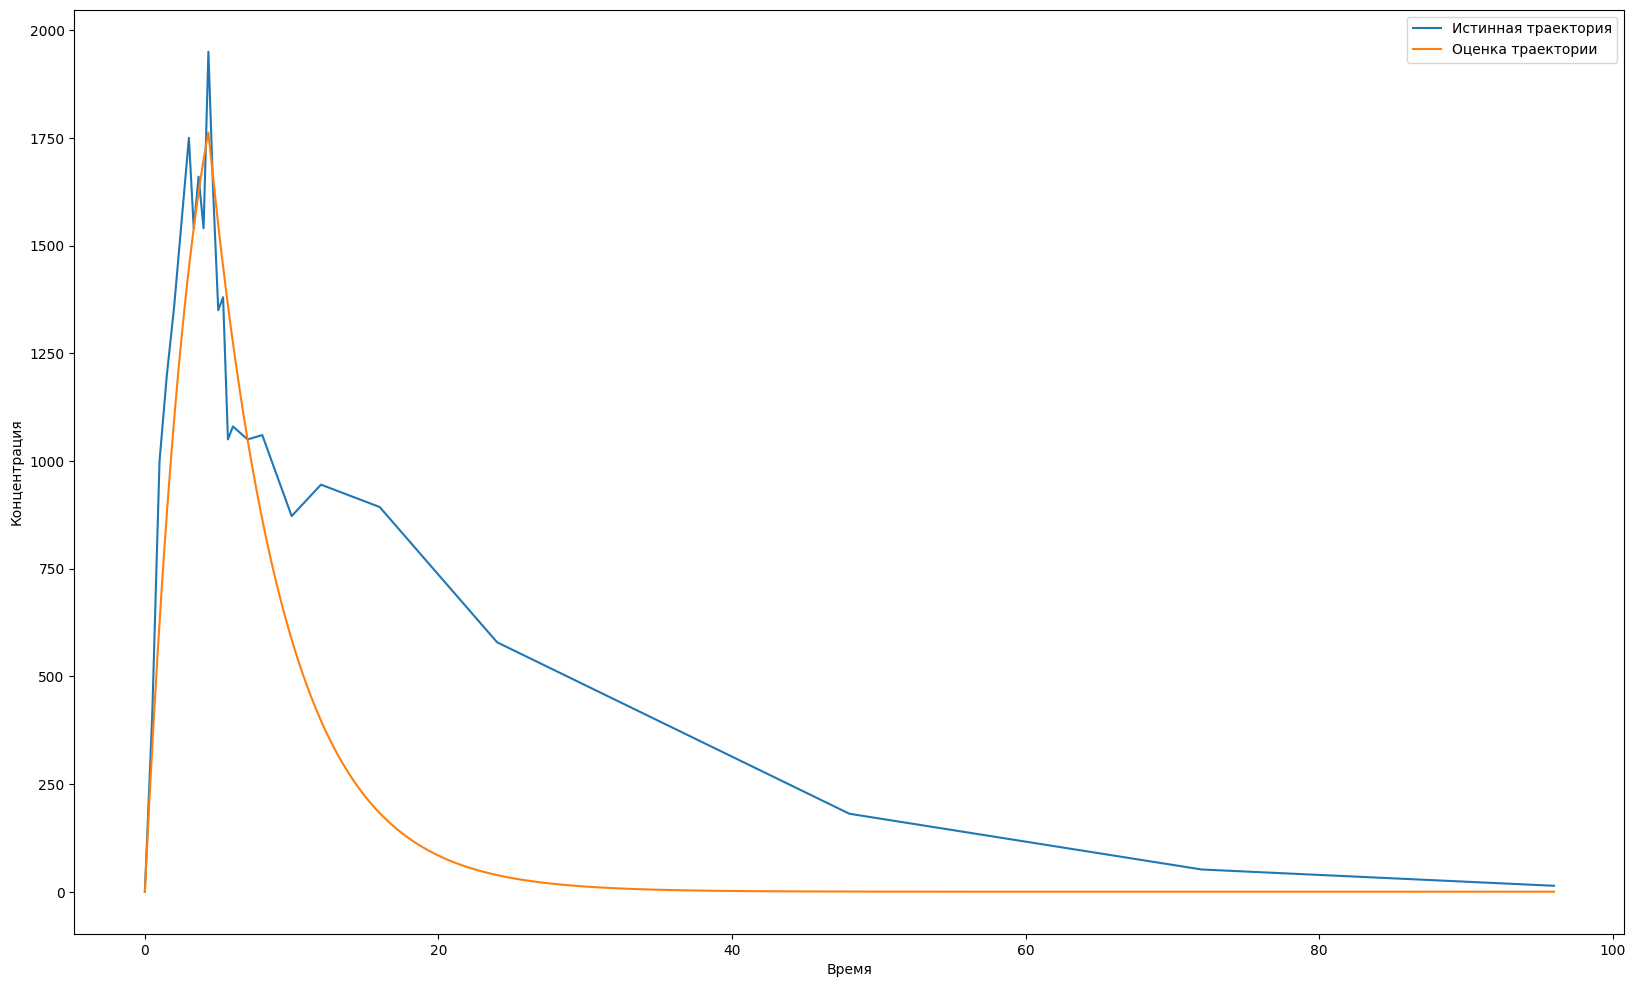
\includegraphics[width=1.0\linewidth]{est.png}
	\caption{Сравнение данных и оценки}
	\label{fig:comparison}
\end{figure}

Хорошо видно, что на этапе абсорбции оценка убывает значительно быстрее нежели истиная траектория, несмотря на то, что на этапе абсорбции оценка показывает неплохую точность.

\section{Описание данных}

Данные были предоставлены Центром научного консультирования и представляют собой синтетические результаты эксперимента по проверке биоэквивалентности двух лекарственных препаратов. Каждый из элементов выборки - временной ряд, отражающий зависимость концентрации активного вещества в крови от времени. Первая выборка - результаты для тестового препарата, вторая - для референтного. Ниже представлены примеры того, как может выглядеть такая кривая.

\begin{figure}[h!]
	\center
	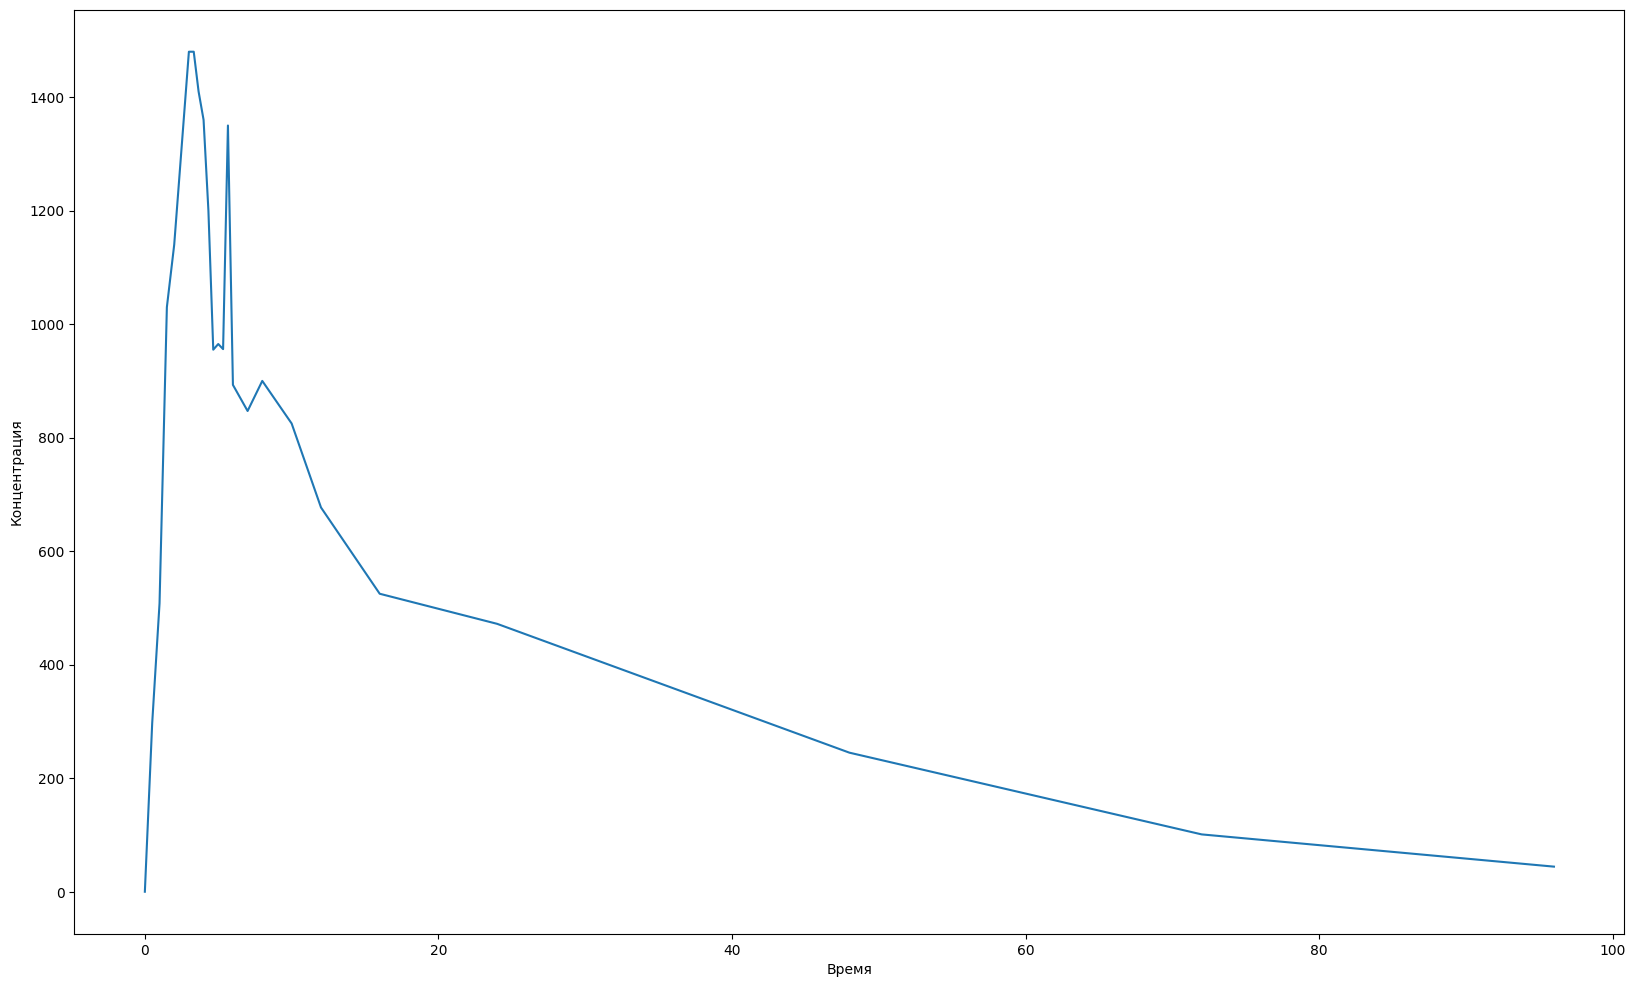
\includegraphics[width=0.9\textwidth]{sample.png}
	\caption{Примеры элементов выборки}
	\label{fig:example}
\end{figure}

Из этого примера можно выделить несколько особенностей, о которых говорилось ранее:

\begin{enumerate}
	\item Невозможность единственным образом оценить $\tau$
	\item Более одного промежутка монотонности
	\item Неоднородность данных по времени
\end{enumerate}

Из-за описанных выше особенностей данных оценка траектории тем методом, которым пользовались авторы оригинальной статьи, является затруднительной.

\newpage

\section{Ансамблирование моделей}

В случае комплексно устроенных лекарственных средств довольно естественным будет следующее предположение: при попадании в организм доза активного вещества по тем или иным причинам разделяется на конечное число различных по своим параметрам доз. Это может происходить как из-за метода действия самого лекарства, так и из-за других менее предсказуемых факторов. При таком подходе наиболее естественной модификаией существующей модели будет ансамблирование нескольких однотипных моделей, у каждой - свой набор параметров. Тогда итоговая оценка траектории будет равна сумме оценок моделей в ансамбле.
Для примера возьмём произвольную траекторию из датасета, построим оценку траектории стандартным методом и рассмотрим остатки:

\begin{figure}[h!]
	\begin{center}
		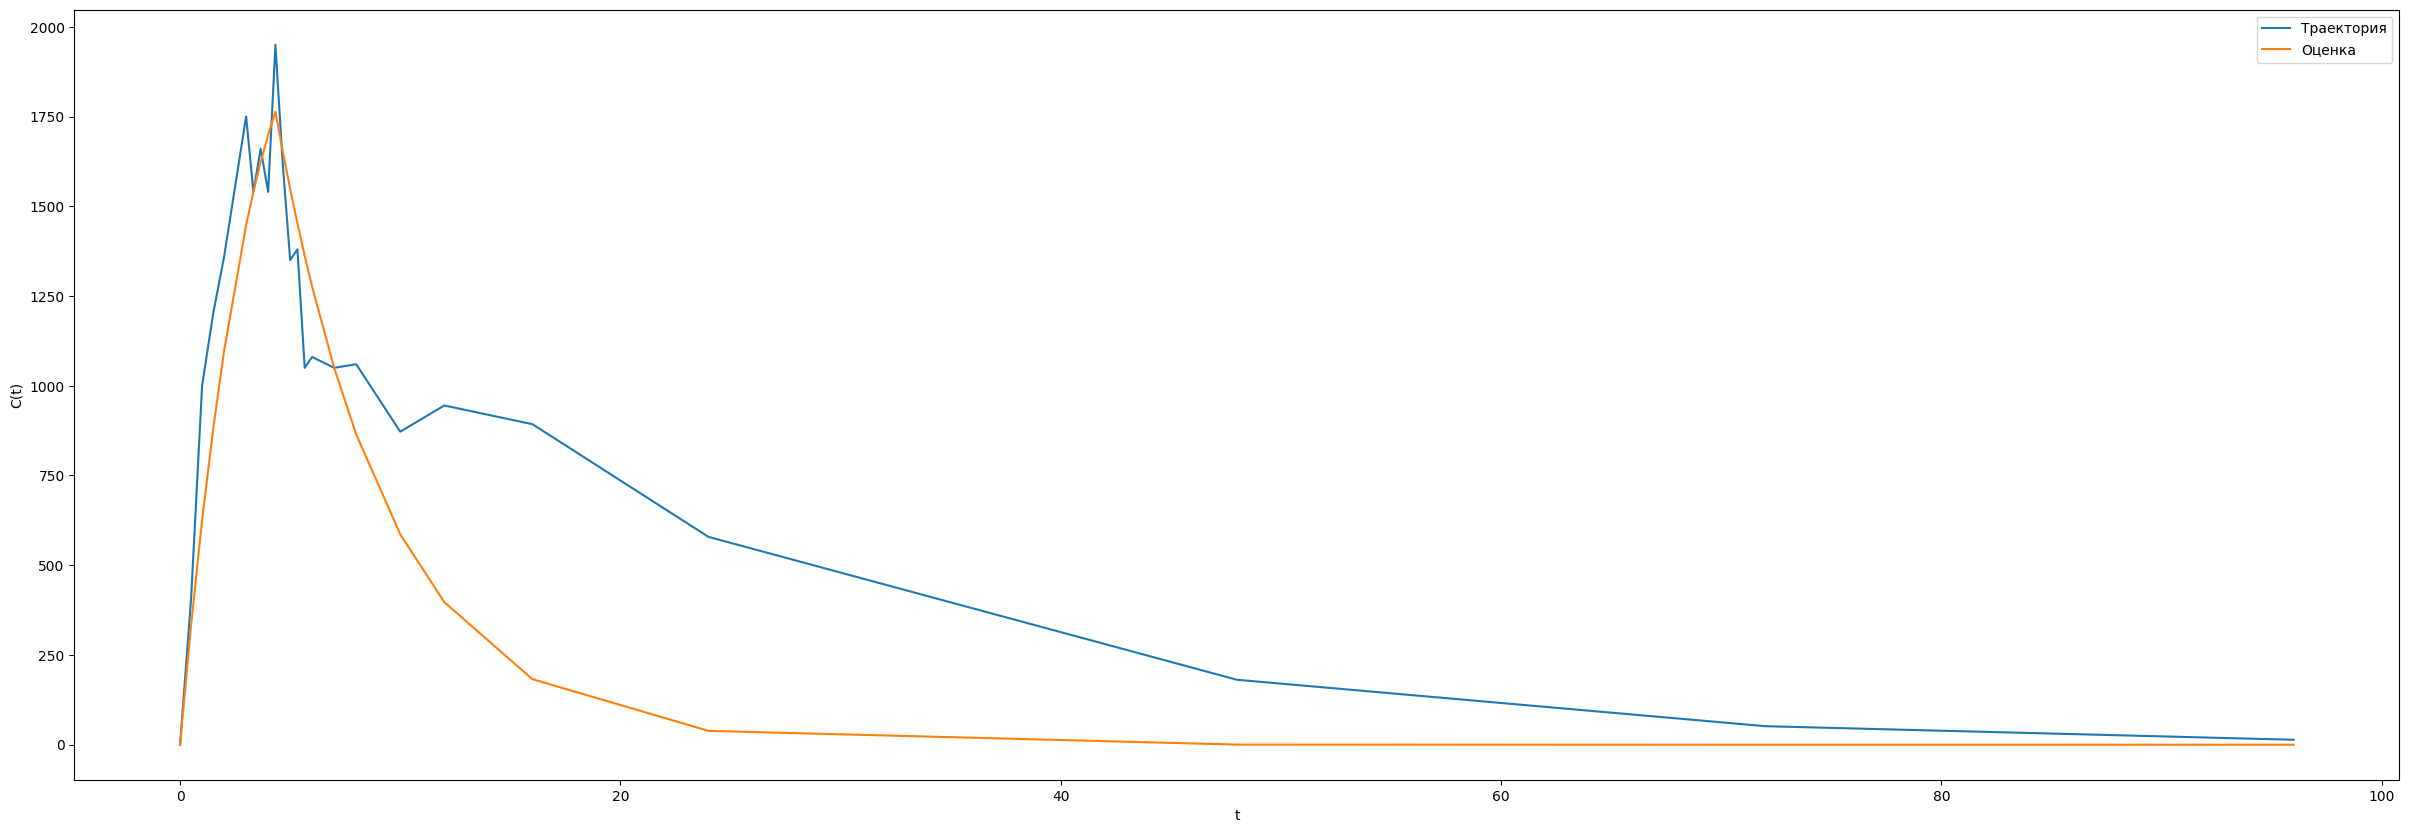
\includegraphics[width=1.0\textwidth]{ensemble/original.png}
		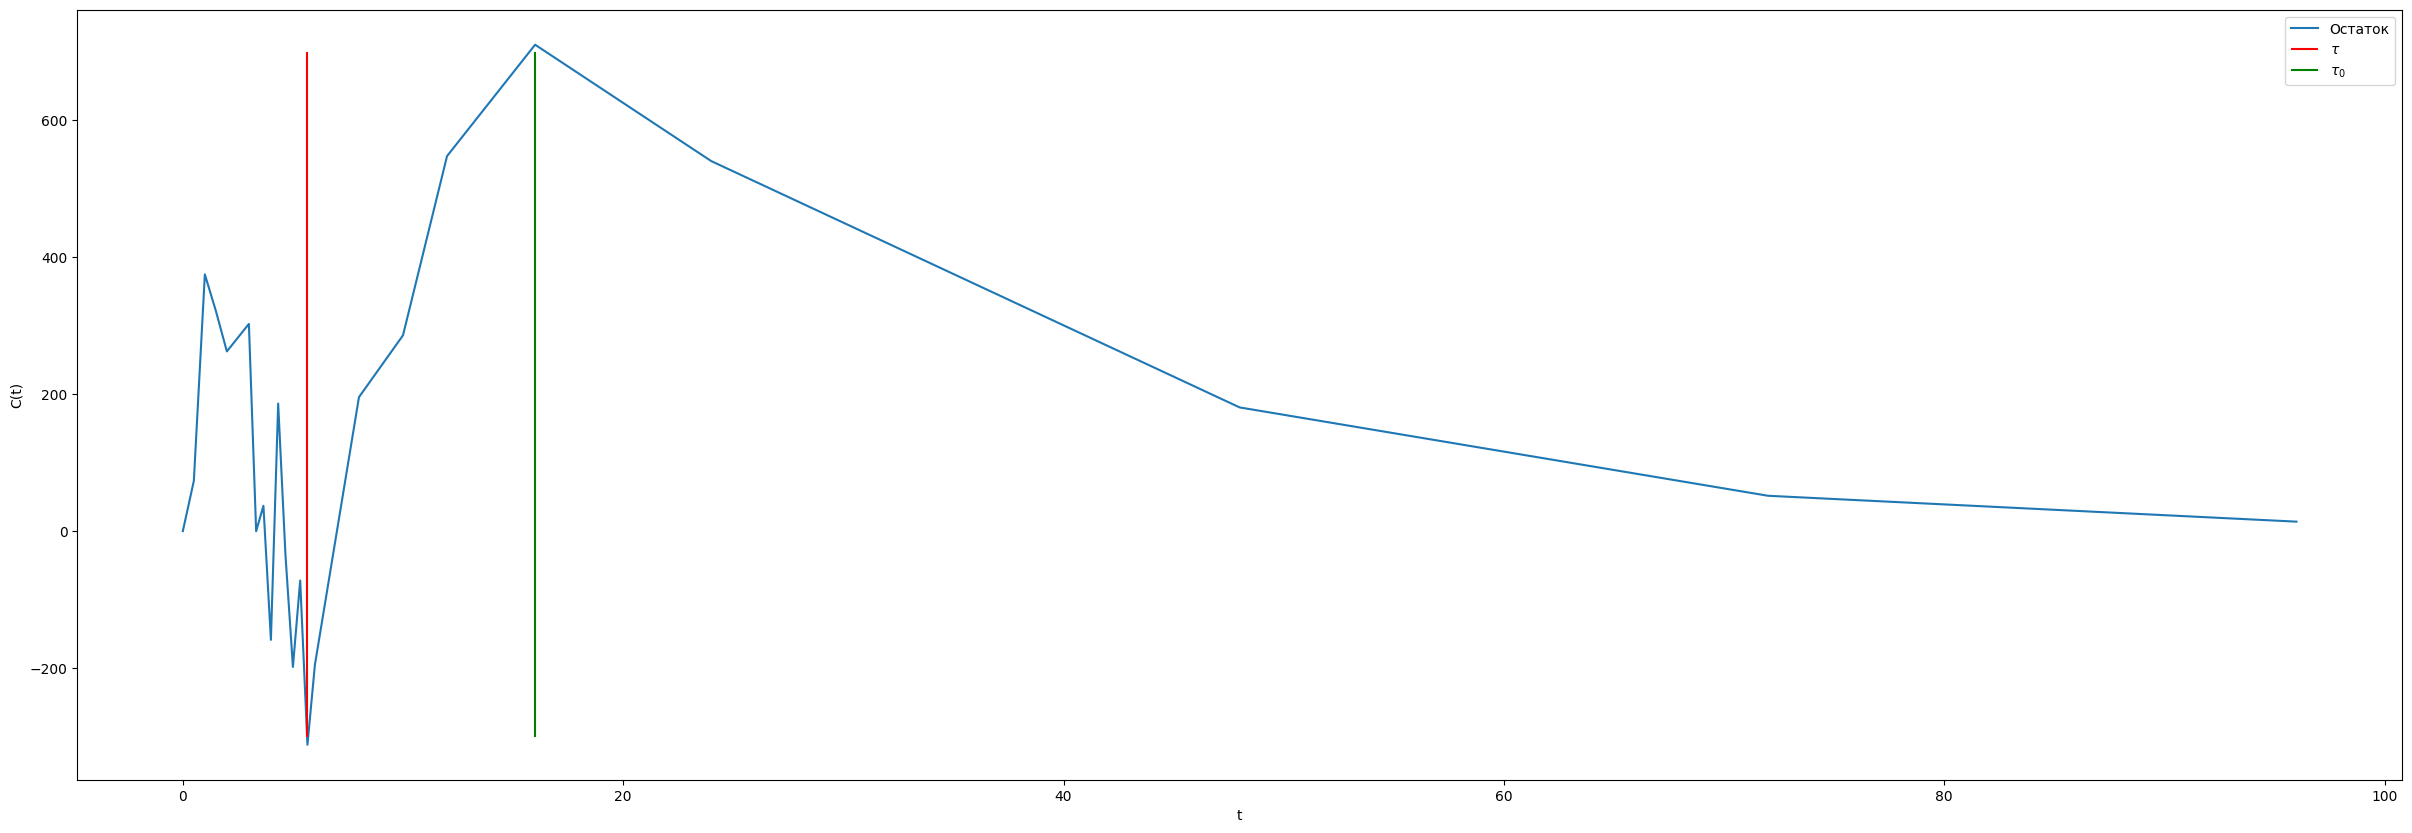
\includegraphics[width=1.0\textwidth]{ensemble/residuals.png}
	\end{center}
	\caption{}\label{fig:res}
\end{figure}
\newpage

Как можно заметить, полученные при оценивании остатки слабо поддаются оцениванию исходным методом. Для исправления этого введём новый параметр $\tau_0$ со следующим физическим смыслом: $\tau_0$ - время, котрое проходит с момента введения до момента начала взаимодействия организма с активным веществом в дозе препарата (на графике отмечено красной вертикальной чертой). В таком случае получаем новую траекторию, где оценка строится на полуинтервале $[\tau_0; +\infty)$, а на отрезке $[0; \tau_0]$ оценка равна нулю.


\subsection{Кусочная модификация PBFTPK}

С учётом описанных выше модификаций, получаем следующий вид функции $C(t)$:

\[
	C(t) = \begin{cases}
		0,                                                                                   & 0 \leq t \le \tau_0 \\
		\frac{FD k_a}{V_d (k_a - k_{el})} (e^{-k_{el}(t - \tau_0)} - e^{-k_a (t - \tau_0)}), & \tau_0 < t \le \tau \\
		C(\tau)e^{-k_{el}((t - \tau_0)-\tau)},                                               & t > \tau
	\end{cases}
\]

\subsection{Методы оценки $\tau$, $\tau_0$}

В оригинальной статье авторами предполагается, что параметр $\tau$ известен. В общем случае эт не так, и более того, при ансамблировании, этот параметр скорее всего будет отличаться у разных компонентов ансамбля. Поскольку эти параметры мы считаем случайными, нужен способ их оценить.

\subsubsection{Минимаксный метод}

\[
	\tau = \argmax_{t_i \in t} C(t_i) \; \; \; \tau_0 = \argmin_{t_i \in t, \; t_i < \tau} C(t_i)
\]

Этот подход является наиболее естественным с точки зрения применения классической модели. Поскольку на этапе абсорбции концентрация растёт, а на этапе элиминации убывает, логично предположить, что и в реальных даных $\tau$ является точкой максимума. Аналогичные рассуждения применимы и к $\tau_0$ - до момента времени $\tau_0$ активное вещество ещё не начало взаимодействовать с организмом, потому и концентрация должна быть минимальна.


\subsubsection{Пиковый метод}

Предыдущий метод зачастую хорошо себя показывает при небольшом количестве моделей в ансамбле и на более <<простых>> траекториях, то есть на тех, на которых в том числе и оригинальная модель показывает довольно неплохие результаты. При использовании ансамблей более удачным будет следующий метод:

\[
	\tau = \max \Argmax_{t_i \in t} C(t_i) \; \; \; \tau_0 = \max \Argmin_{t_i \in t, \; t_i < \tau} C(t_i)
\]

Идея этого метода заключается в следующем - модель сначала находит тут компоненту лекарства, которая позже остальных начала своё взаимодействие. В качестве остатка получается траектория, имеющая на 1 пик меньше. Благодаря этому следующая модель в ансамбле, действуя по похожему алгоритму, ещё больше сглаживает траекторию. Таким образом, с каждой итерацией по ансамблю модель получает всё более близкие по евклидовой норме к нулю остатки.

\todo{Вставить серию картинок со сглаживанием траектории}

\section{Модификация функции потерь}

В оригинальной статье авторы в качестве функции потерь используют стандартную среднеквадратичную функцию потерь (\textbf{MSE}). Основной проблемой использования такой функции в реальных данных является обозначенная выше неоднородность данных по времени. Поскольку в окрестности $\tau$ наблюдений зачастую гораздо больше, полученная с помощью такой функции потерь оценка также будет наиболее точна в окрестности $\tau$. Чтобы это исправить, используем следующую функцию потерь:

\[
	L_{\lambda}(t, C, \hat{C}) = \frac{1}{\#(t)}\sum_{t_i \in t} \Big(C(t_i)-\hat{C}(t_i)\Big)^2 \cdot
	\begin{cases}
		1,       & t_i \le \tau \\
		\lambda, & t_i > \tau
	\end{cases}
\]

Такую функцию будем называть \textbf{$\lambda$-взвешенной среднеквадратичной функцией потерь} ($\textbf{WMSE}_{\lambda}$). Параметр $\lambda$ для такой функции можно задавать по-разному. Наиболее естественным будет следюущий способ: $\lambda = \frac{\# \{t_i \in t | t_i \le \tau \}}{\# \{ t_i \in t | t_i > \tau \}}$. Естественность этого подхода заключается в том, что в таком случае нивелируется влияние большого количества наблюдений на этапе абсорбции по отношению к количеству набблюдений на этапе элиминации.

\section{Заключение}

Бла бла бла.

\bibliographystyle{gost780u.bst} % Для соответствия требованиям об оформлении списка литературы
\raggedright
\bibliography{references}

% Раскомментируйте, если нужно приложение
% \appendix

% \cleardoublepage \phantomsection
% \section*{Приложение}
% \addcontentsline{toc}{section}{Приложение}

\end{document}
